\qrchapter{https://forgottenpillar.com/rsc/en-fp-chapter1}{The Foundation of Our Faith}


\qrchapter{https://forgottenpillar.com/rsc/en-fp-chapter1}{أساس إيماننا}


\egw{\textbf{The Lord will put new, vital force into His work} as human agencies obey the command to go forth and proclaim the truth. \textbf{He who declared that His truth would shine forever will proclaim this truth through faithful messengers, who will give the trumpet a certain sound}. \textbf{The truth will be criticized, scorned, and derided; but the \underline{closer} it is examined and tested, \underline{the brighter it will shine}}.}[SpTB02 51.1; 1904][https://egwwritings.org/read?panels=p417.260]


\egw{\textbf{سيضع الرب قوة جديدة وحيوية في عمله} عندما تطيع الوسائل البشرية الأمر بالخروج وإعلان الحق. \textbf{إن الذي أعلن أن حقه سيشرق إلى الأبد سيعلن هذا الحق من خلال رسل أمناء، سيعطون البوق صوتًا واضحًا}. \textbf{سيتم انتقاد الحق والسخرية منه والاستهزاء به؛ ولكن \underline{كلما} تم فحصه واختباره عن قرب، \underline{كلما سطع بشكل أكثر إشراقًا}}.}[SpTB02 51.1; 1904][https://egwwritings.org/read?panels=p417.260]


\egwnogap{\textbf{As a people, we are to \underline{stand firm on the platform of eternal truth} that has withstood test and trial. We are to \underline{hold to the sure pillars of our faith}. The \underline{principles of truth} that God has revealed to us \underline{are our only true foundation}. They have made us what we are. The lapse of time has not lessened their value. \underline{It is the constant effort of the enemy to remove these truths from their setting}, and to put in their place \underline{spurious theories}. He \underline{will bring in} everything that he possibly can to carry out his deceptive designs. But the Lord will raise up men of keen perception, who will give these truths their proper place in the plan of God.}}[SpTB02 51.2; 1904][https://egwwritings.org/read?panels=p417.261]


\egwnogap{\textbf{كشعب، علينا أن \underline{نقف بثبات على منصة الحق الأبدي} التي صمدت أمام الاختبار والتجربة. علينا أن \underline{نتمسك بالأعمدة الثابتة لإيماننا}. إن \underline{مبادئ الحق} التي كشفها الله لنا \underline{هي أساسنا الحقيقي الوحيد}. لقد جعلتنا ما نحن عليه. لم يقلل مرور الوقت من قيمتها. \underline{إنه الجهد المستمر للعدو لإزالة هذه الحقائق من موضعها}، ووضع \underline{نظريات زائفة} مكانها. سوف \underline{يُدخل} كل ما يمكنه لتنفيذ مخططاته الخادعة. لكن الرب سيقيم رجالاً ذوي بصيرة حادة، سيضعون هذه الحقائق في مكانها الصحيح في خطة الله.}}[SpTB02 51.2; 1904][https://egwwritings.org/read?panels=p417.261]


\egwnogap{\textbf{I have been instructed by the heavenly messenger that some of the reasoning in the book, ‘Living Temple,’ is unsound and that \underline{this reasoning would lead astray} the minds of those who are not thoroughly established on \underline{the foundation principles} of present truth. It introduces that which is naught but speculation in \underline{regard to the personality of God and where His presence is}}. No one on this earth has a right to speculate on this question. \textbf{The more fanciful theories are discussed, the less men will know of God and of the truth that sanctifies the soul}.}[SpTB02 51.3; 1904][https://egwwritings.org/read?panels=p417.262]


\egwnogap{\textbf{لقد تلقيت تعليمات من الرسول السماوي بأن بعض المنطق في كتاب “ذا ليفينغ تمبل” غير سليم وأن \underline{هذا المنطق سيضلل} عقول أولئك الذين ليسوا راسخين تمامًا على \underline{المبادئ الأساسية} للحق الحاضر. إنه يقدم ما هو مجرد تكهنات \underline{فيما يتعلق بشخصانية الله وأين يوجد حضوره}}. ليس لأحد على هذه الأرض الحق في التكهن حول هذه المسألة. \textbf{كلما نوقشت النظريات الخيالية، قل ما سيعرفه الناس عن الله وعن الحق الذي يقدس النفس}.}[SpTB02 51.3; 1904][https://egwwritings.org/read?panels=p417.262]


\egwnogap{One and another come to me, asking me \textbf{to explain the positions taken in ‘Living Temple.’} I reply, ‘\textbf{They are unexplainable}.’ \textbf{The sentiments expressed do not give a true knowledge of God}. All through the book are passages of scripture. These scriptures are brought in in such a way that error is made to appear as truth. \textbf{Erroneous theories are presented in so pleasing a way that unless care is taken, many will be misled}.}[SpTB02 52.1; 1904][https://egwwritings.org/read?panels=p417.265]


\egwnogap{يأتي إليّ واحد تلو الآخر، يسألني \textbf{أن أشرح المواقف المتخذة في “ذا ليفينغ تمبل”.} أجيب، “\textbf{إنها غير قابلة للشرح}.” \textbf{الآراء المعبر عنها لا تعطي معرفة حقيقية بالله}. في جميع أنحاء الكتاب توجد مقاطع من الكتاب المقدس. تم إدراج هذه النصوص الكتابية بطريقة تجعل الخطأ يبدو كأنه حقيقة. \textbf{يتم تقديم النظريات الخاطئة بطريقة جذابة لدرجة أنه ما لم يتم توخي الحذر، سيضل الكثيرون}.}[SpTB02 52.1; 1904][https://egwwritings.org/read?panels=p417.265]


\egwnogap{\textbf{We need not the mysticism that is in this book}. Those who entertain these sophistries will soon find themselves in a position where the enemy can talk with them, and lead them away from God. It is represented to me that the writer of this book is on a false track. \textbf{He has lost sight of the distinguishing truths for \underline{this time}}. He knows not whither his steps are tending. \textbf{\underline{The track of truth lies close beside the track of error}, and both tracks may seem to be one to minds which are not worked by the Holy Spirit, and which, therefore, are not quick to discern the difference between truth and error}.}[SpTB02 52.2; 1904][https://egwwritings.org/read?panels=p417.266]


\egwnogap{\textbf{نحن لسنا بحاجة إلى الصوفية الموجودة في هذا الكتاب}. أولئك الذين يتبنون هذه السفسطات سيجدون أنفسهم قريبًا في موقف يمكن للعدو أن يتحدث معهم فيه، ويبعدهم عن الله. لقد تم تمثيله لي أن كاتب هذا الكتاب على مسار خاطئ. \textbf{لقد فقد رؤية الحقائق المميزة \underline{لهذا الوقت}}. إنه لا يعرف إلى أين تتجه خطواته. \textbf{\underline{إن مسار الحق يقع بالقرب من مسار الخطأ}، وقد يبدو كلا المسارين واحدًا للعقول التي لا يعمل فيها الروح القدس، والتي، بالتالي، ليست سريعة في إدراك الفرق بين الحق والخطأ}.}[SpTB02 52.2; 1904][https://egwwritings.org/read?panels=p417.266]


\egwnogap{\textbf{About the time that ‘Living Temple’ was published, there passed before me in the night season, \underline{representations indicating that some danger was approaching}, and that I must prepare for it by \underline{writing out the things} God has revealed to me \underline{regarding the foundation principles of our faith}}.}[SpTB02 52.3; 1904][https://egwwritings.org/read?panels=p417.267]


\egwnogap{\textbf{في حوالي وقت نشر “ذا ليفينغ تمبل”، مرت أمامي في ساعات الليل، \underline{تمثيلات تشير إلى أن بعض الخطر كان يقترب}، وأنه يجب أن أستعد له من خلال \underline{كتابة الأشياء} التي كشفها الله لي \underline{بخصوص المبادئ الأساسية لإيماننا}}.}[SpTB02 52.3; 1904][https://egwwritings.org/read?panels=p417.267]


\egwnogap{A copy of ‘Living Temple’ was sent me, but it remained in my library, unread. From the light given me by the Lord, \textbf{I knew that some of the sentiments advocated in the book, did not bear the indorsement of God}, \textbf{and that they were \underline{a snare that the enemy had prepared for the last days}}. I thought that this would surely be discerned, and that it would not be necessary for me to say anything about it.}[SpTB02 52.4; 1904][https://egwwritings.org/read?panels=p417.268]


\egwnogap{تم إرسال نسخة من “ذا ليفينغ تمبل” إلي، لكنها بقيت في مكتبتي، دون أن تُقرأ. من النور الذي أعطاني إياه الرب، \textbf{عرفت أن بعض الآراء التي يدافع عنها الكتاب، لم تحمل مصادقة الله}، \textbf{وأنها كانت \underline{فخًا أعده العدو للأيام الأخيرة}}. اعتقدت أنه سيتم إدراك هذا بالتأكيد، وأنه لن يكون من الضروري أن أقول أي شيء عنه.}[SpTB02 52.4; 1904][https://egwwritings.org/read?panels=p417.268]


\egwnogap{In the controversy that arose among our brethren \textbf{regarding the teachings of this book}, those in favor of giving it a wide circulation declared: ‘\textbf{It contains the very sentiments that Sister White has been teaching}.’ This assertion struck right to my heart. I felt heart-broken; for \textbf{I knew that this representation of the matter \underline{was not true}}.}[SpTB02 53.1; 1904][https://egwwritings.org/read?panels=p417.270]


\egwnogap{في الجدل الذي نشأ بين إخوتنا \textbf{بخصوص تعاليم هذا الكتاب}، أعلن المؤيدون لإعطائه انتشارًا واسعًا: “\textbf{إنه يحتوي على نفس الآراء التي كانت الأخت وايت تعلّمها}.” هذا التأكيد ضرب قلبي مباشرة. شعرت بانكسار القلب؛ لأنني \textbf{عرفت أن هذا التمثيل للأمر \underline{لم يكن صحيحًا}}.}[SpTB02 53.1; 1904][https://egwwritings.org/read?panels=p417.270]


\egwnogap{Finally my son said to me, ‘Mother, you ought to read at least some parts of the book, that you may see whether they are in harmony with the light that God has given you.’ He sat down beside me, and together \textbf{we read the preface, and most of the first chapter, and also paragraphs in other chapters}. As we read, I recognized the very sentiments against which I had been bidden to speak in warning \textbf{during \underline{the early days} of my public labors}. When I first left the State of Maine, it was to go through Vermont and Massachusetts, to bear a testimony against these sentiments. \textbf{‘Living Temple’ contains the alpha of these theories. I knew that the \underline{omega would follow in a little while}; and I trembled for our people}. \textbf{I knew that I must warn our brethren and sisters not to enter into controversy \underline{over the presence and personality of God}}. \textbf{The statements made in ‘Living Temple’ \underline{in regard to this point are incorrect}}. The scripture used to substantiate the doctrine there set forth, is scripture misapplied.}[SpTB02 53.2; 1904][https://egwwritings.org/read?panels=p417.271]


\egwnogap{أخيرًا قال لي ابني، “أمي، يجب أن تقرئي على الأقل بعض أجزاء الكتاب، لترى ما إذا كانت متوافقة مع النور الذي أعطاك الله إياه.” جلس بجانبي، وسويًا \textbf{قرأنا المقدمة، ومعظم الفصل الأول، وكذلك فقرات في فصول أخرى}. أثناء القراءة، تعرفت على نفس الآراء التي أُمرت بالتحدث ضدها في تحذير \textbf{خلال \underline{الأيام الأولى} من خدمتي العامة}. عندما غادرت ولاية مين لأول مرة، كان ذلك للذهاب عبر فيرمونت وماساتشوستس، لأحمل شهادة ضد هذه الآراء. \textbf{يحتوي “ذا ليفينغ تمبل” على ألفا هذه النظريات. كنت أعلم أن \underline{الأوميغا ستتبع بعد قليل}؛ وارتعدت من أجل شعبنا}. \textbf{عرفت أنه يجب أن أحذر إخوتنا وأخواتنا من الدخول في جدل \underline{حول حضور وشخصانية الله}}. \textbf{البيانات الواردة في “ذا ليفينغ تمبل” \underline{فيما يتعلق بهذه النقطة غير صحيحة}}. الكتاب المقدس المستخدم لدعم العقيدة المطروحة هناك، هو كتاب مقدس مطبق بشكل خاطئ.}[SpTB02 53.2; 1904][https://egwwritings.org/read?panels=p417.271]


\egwnogap{\textbf{I am compelled to speak in denial of the claim that the teachings of ‘Living Temple’ can be sustained by statements from my writings}. \textbf{There may be in this book expressions and sentiments that are in harmony with my writings}. \textbf{And there may be in my writings many statements which, taken from their connection, and interpreted according to the mind of the writer of ‘Living Temple,’ would seem to be in harmony with the teachings of this book.} This may give apparent support to the assertion that the sentiments in ‘Living Temple’ are in harmony with my writings. \textbf{But God forbid that this sentiment should prevail}.}[SpTB02 53.3; 1904][https://egwwritings.org/read?panels=p417.272]


\egwnogap{\textbf{أنا مضطرة للتحدث لإنكار الادعاء بأن تعاليم ‘ذا ليفينغ تمبل’ يمكن دعمها بعبارات من كتاباتي}. \textbf{قد تكون في هذا الكتاب تعبيرات وآراء متناغمة مع كتاباتي}. \textbf{وقد تكون في كتاباتي عبارات كثيرة، إذا أُخذت من سياقها، وفُسرت وفقًا لعقل كاتب ‘ذا ليفينغ تمبل’، قد تبدو متناغمة مع تعاليم هذا الكتاب.} هذا قد يعطي دعمًا ظاهريًا للتأكيد بأن الآراء في ‘ذا ليفينغ تمبل’ متناغمة مع كتاباتي. \textbf{لكن حاشا لله أن يسود هذا الرأي}.}[SpTB02 53.3; 1904][https://egwwritings.org/read?panels=p417.272]


\egwnogap{\textbf{Few can discern the result of entertaining the sophistries advocated by some at this time}. \textbf{But the Lord has lifted the curtain, and has \underline{shown me the result that would follow}}. \textbf{The spiritualistic theories \underline{regarding the personality of God}, followed to their logical conclusion, sweep away the whole Christian economy}. \textbf{They estimate as nothing the light that Christ came from heaven to give John to give to His people. They teach that the scenes just before us are not of sufficient importance to be given special attention. They make of no effect the truth of heavenly origin, \underline{and rob the people of God of their past experience}, giving them instead a false science}.}[SpTB02 54.1; 1904][https://egwwritings.org/read?panels=p417.275]


\egwnogap{\textbf{قليلون هم الذين يستطيعون تمييز نتيجة تبني السفسطات التي يدعو إليها البعض في هذا الوقت}. \textbf{لكن الرب رفع الستار، و\underline{أراني النتيجة التي ستتبع}}. \textbf{النظريات الروحانية \underline{المتعلقة بشخصانية الله}، إذا اتبعت إلى نتائجها المنطقية، تجرف النظام المسيحي بأكمله}. \textbf{إنهم لا يقدرون النور الذي جاء به المسيح من السماء ليعطيه ليوحنا ليعطيه لشعبه. يعلّمون أن المشاهد التي أمامنا مباشرة ليست ذات أهمية كافية لإعطائها اهتمامًا خاصًا. إنهم يجعلون الحق ذا الأصل السماوي بلا تأثير، \underline{ويسلبون شعب الله تجربتهم الماضية}، ويعطونهم بدلاً منها علمًا زائفًا}.}[SpTB02 54.1; 1904][https://egwwritings.org/read?panels=p417.275]


\egwnogap{\textbf{In a vision} of the night I was shown distinctly that \textbf{these sentiments} have been looked upon by some as \textbf{the grand truths} \textbf{that are to be \underline{brought in}} and made prominent at the present time. \textbf{I was shown \underline{a platform}, braced by \underline{solid timbers},—the truths of the Word of God}. \textbf{Some one high in responsibility in the medical work was directing this man and that man to loosen the timbers supporting this platform}. Then I heard a voice saying, ‘Where are the watchmen that ought to be standing on the walls of Zion? Are they asleep? \textbf{\underline{This foundation was built by the Masterworker}, and \underline{will} stand storm and tempest. Will they permit this man to \underline{present doctrines} \underline{that deny the past experience} of the people of God? The time has come to take decided action}.’}[SpTB02 54.2; 1904][https://egwwritings.org/read?panels=p417.276]


\egwnogap{\textbf{في رؤيا} الليل أُريت بوضوح أن \textbf{هذه الآراء} قد نظر إليها البعض على أنها \textbf{الحقائق العظيمة} \textbf{التي يجب \underline{إدخالها}} وإبرازها في الوقت الحاضر. \textbf{رأيت \underline{منصة}، مدعمة \underline{بأخشاب صلبة}،—حقائق كلمة الله}. \textbf{كان شخص ما ذو مسؤولية عالية في العمل الطبي يوجه هذا الرجل وذاك الرجل لتخفيف الأخشاب التي تدعم هذه المنصة}. ثم سمعت صوتًا يقول، ‘أين الحراس الذين ينبغي أن يقفوا على أسوار صهيون؟ أهم نائمون؟ \textbf{\underline{هذا الأساس بناه العامل الرئيسي}، و\underline{سيصمد} أمام العاصفة والزوبعة. هل سيسمحون لهذا الرجل \underline{بتقديم عقائد} \underline{تنكر التجربة الماضية} لشعب الله؟ لقد حان وقت اتخاذ إجراء حاسم}.’}[SpTB02 54.2; 1904][https://egwwritings.org/read?panels=p417.276]


\egwnogap{\textbf{The enemy of souls has sought to \underline{bring in} the supposition that \underline{a great reformation} was to take place among Seventh-day Adventists, and that \underline{this reformation} would \underline{consist in giving up the doctrines which stand as the pillars of our faith,} and engaging in a process of reorganization}. \textbf{Were this reformation to take place, \underline{what would result}?} \textbf{\underline{The principles of truth} that God in His wisdom has given to the remnant church, \underline{would be discarded}}. \textbf{Our religion would be changed}. \textbf{\underline{The fundamental principles} that have sustained the work for the last fifty years \underline{would be accounted as error}}. \textbf{A new organization would be established}. \textbf{Books of a new order would be written}.\textbf{ A system of intellectual philosophy would be introduced}. The founders of this system would go into the cities, and do a wonderful work. The Sabbath, of course, would be lightly regarded, \textbf{as also the God who created it}. Nothing would be allowed to stand in the way of the new movement. \textbf{The leaders would teach that virtue is better than vice, but God being removed, they would place their dependence on human power, which, without God, is worthless}. \textbf{Their foundation would be built on the sand, and storm and tempest would sweep away the structure}.}[SpTB02 54.3; 1904][https://egwwritings.org/read?panels=p417.277]


\egwnogap{\textbf{سعى عدو النفوس \underline{لإدخال} افتراض أن \underline{إصلاحًا عظيمًا} كان سيحدث بين الأدفنتست السبتيين، وأن \underline{هذا الإصلاح} سوف \underline{يتألف من التخلي عن العقائد التي تقف كأعمدة إيماننا،} والانخراط في عملية إعادة تنظيم}. \textbf{لو حدث هذا الإصلاح، \underline{ماذا ستكون النتيجة}؟} \textbf{\underline{مبادئ الحق} التي أعطاها الله في حكمته للكنيسة الباقية، \underline{ستُرفض}}. \textbf{ستتغير ديانتنا}. \textbf{\underline{المبادئ الجوهرية} التي دعمت العمل خلال الخمسين سنة الماضية \underline{ستُعتبر خطأ}}. \textbf{ستُؤسس منظمة جديدة}. \textbf{ستُكتب كتب من نوع جديد}. \textbf{سيُقدم نظام للفلسفة الفكرية}. مؤسسو هذا النظام سيذهبون إلى المدن، ويقومون بعمل رائع. السبت، بالطبع، سيُعتبر بشكل خفيف، \textbf{وكذلك الله الذي خلقه}. لن يُسمح لأي شيء بالوقوف في طريق الحركة الجديدة. \textbf{سيعلّم القادة أن الفضيلة أفضل من الرذيلة، لكن مع إزالة الله، سيضعون اعتمادهم على القوة البشرية، التي بدون الله، لا قيمة لها}. \textbf{سيُبنى أساسهم على الرمل، وستجرف العاصفة والزوبعة البنيان}.}[SpTB02 54.3; 1904][https://egwwritings.org/read?panels=p417.277]


\egwnogap{Who has authority to begin such a movement? \textbf{We have our Bibles}. \textbf{We have our experience, attested to by the miraculous working of the Holy Spirit}. \textbf{We have a truth that admits of no compromise}. \textbf{\underline{Shall we not repudiate everything that is not in harmony with this truth}}?}[SpTB02 55.1; 1904][https://egwwritings.org/read?panels=p417.280]


\egwnogap{من لديه السلطة لبدء مثل هذه الحركة؟ \textbf{لدينا كتبنا المقدسة}. \textbf{لدينا تجربتنا، مؤيدة بالعمل المعجزي للروح القدس}. \textbf{لدينا حق لا يقبل المساومة}. \textbf{\underline{ألا يجب أن نرفض كل ما ليس متناغمًا مع هذا الحق}}؟}[SpTB02 55.1; 1904][https://egwwritings.org/read?panels=p417.280]


\egwnogap{I hesitated and delayed about the sending out of that which the Spirit of the Lord impelled me to write. \textbf{I did not want to be compelled to present the misleading influence of these sophistries. But in the providence of God, the errors that have been coming in must be met}.}[SpTB02 55.2; 1904][https://egwwritings.org/read?panels=p417.281]


\egwnogap{ترددت وتأخرت في إرسال ما دفعني روح الرب لكتابته. \textbf{لم أرغب في أن أُجبر على تقديم التأثير المضلل لهذه السفسطات. لكن في عناية الله، يجب مواجهة الأخطاء التي كانت تدخل}.}[SpTB02 55.2; 1904][https://egwwritings.org/read?panels=p417.281]


\egwnogap{Shortly before \textbf{I sent out the testimonies regarding the \underline{efforts of the enemy to undermine the foundation of our faith} through the dissemination of \underline{seductive theories}}, I had read an incident about a ship in a fog meeting an iceberg. For several nights I slept but little. I seemed to be bowed down as a cart beneath sheaves. One night a scene was clearly presented before me. A vessel was upon the waters, in a heavy fog. Suddenly the lookout cried, ‘Iceberg just ahead!’ There, towering high above the ship, was a gigantic iceberg. An authoritative voice cried out, ‘Meet it!’ There was not a moment’s hesitation. It was a time for instant action. The engineer put on full steam, and the man at the wheel steered the ship straight into the iceberg. With a crash she struck the ice. There was a fearful shock, and the iceberg broke into many pieces, falling with a noise like thunder to the deck. The passengers were violently shaken by the force of the collision, but no lives were lost. The vessel was injured, but not beyond repair. She rebounded from the contact, trembling from stem to stern, like a living creature. Then she moved forward on her way.}[SpTB02 55.3; 1904][https://egwwritings.org/read?panels=p417.282]


\egwnogap{قبل وقت قصير من \textbf{إرسالي للشهادات المتعلقة \underline{بجهود العدو لتقويض أساس إيماننا} من خلال نشر \underline{نظريات مغرية}}، قرأت حادثة عن سفينة في ضباب تصطدم بجبل جليدي. لعدة ليالٍ نمت قليلاً. بدا كأنني منحنية كعربة تحت حزم. في إحدى الليالي، عُرض أمامي مشهد بوضوح. كانت سفينة على المياه، في ضباب كثيف. فجأة صرخ المراقب، ‘جبل جليدي مباشرة في المقدمة!’ هناك، مرتفعًا عاليًا فوق السفينة، كان جبل جليدي ضخم. صرخ صوت ذو سلطة، ‘واجهه!’ لم يكن هناك لحظة تردد. كان وقتًا للعمل الفوري. وضع المهندس البخار الكامل، ووجه الرجل عند العجلة السفينة مباشرة نحو الجبل الجليدي. بصوت تحطم اصطدمت بالجليد. كانت هناك صدمة مخيفة، وتكسر الجبل الجليدي إلى قطع كثيرة، سقطت بصوت كالرعد على السطح. اهتز الركاب بعنف من قوة الاصطدام، لكن لم تُفقد أرواح. تضررت السفينة، لكن ليس بما يتجاوز الإصلاح. ارتدت من الاتصال، ترتجف من المقدمة إلى المؤخرة، مثل مخلوق حي. ثم تحركت للأمام في طريقها.}[SpTB02 55.3; 1904][https://egwwritings.org/read?panels=p417.282]


\egwnogap{Well I knew the meaning of this representation. \textbf{I had my orders}. I had heard the words, like a voice from our Captain, ‘\textbf{Meet it}!’ I knew what my duty was, and that there was not a moment to lose. The time for decided action had come. \textbf{I must without delay obey the command, ‘Meet it!’}}[SpTB02 56.1; 1904][https://egwwritings.org/read?panels=p417.285]


\egwnogap{عرفت جيدًا معنى هذا التمثيل. \textbf{كانت لدي أوامري}. سمعت الكلمات، مثل صوت من قائدنا، ‘\textbf{واجهه}!’ عرفت ما هو واجبي، وأنه لم يكن هناك لحظة لأضيعها. جاء وقت العمل الحاسم. \textbf{يجب أن أطيع الأمر دون تأخير، ‘واجهه!’}}[SpTB02 56.1; 1904][https://egwwritings.org/read?panels=p417.285]


\egwnogap{That night I was up at one o’clock, writing as fast as my hand could pass over the paper. For the next few days I worked early and late, \textbf{preparing for our people the instruction given me \underline{regarding the errors} that were \underline{coming in} among us}.}[SpTB02 56.2; 1904][https://egwwritings.org/read?panels=p417.286]


\egwnogap{تلك الليلة كنت مستيقظة في الساعة الواحدة، أكتب بسرعة قدر ما تستطيع يدي أن تمر على الورق. خلال الأيام القليلة التالية عملت مبكرًا ومتأخرًا، \textbf{أعد لشعبنا التعليمات التي أُعطيت لي \underline{بخصوص الأخطاء} التي كانت \underline{تدخل} بيننا}.}[SpTB02 56.2; 1904][https://egwwritings.org/read?panels=p417.286]


\egwnogap{\textbf{I have been hoping that there would be a thorough reformation, and that \underline{the principles} for which we fought \underline{in the early days}, and which were brought out in the power of the Holy Spirit, \underline{would be maintained}}.}[SpTB02 56.3; 1904][https://egwwritings.org/read?panels=p417.287]


\egwnogap{\textbf{كنت آمل أن يكون هناك إصلاح شامل، وأن \underline{المبادئ} التي حاربنا من أجلها \underline{في الأيام الأولى}، والتي أُخرجت بقوة الروح القدس، \underline{ستُحافظ عليها}}.}[SpTB02 56.3; 1904][https://egwwritings.org/read?panels=p417.287]


\egwnogap{\textbf{Many of our people do not realize \underline{how firmly} the foundation of our faith has been laid}. \textbf{My husband, Elder Joseph Bates, Father Pierce, Elder Edson, and others who were keen, noble, and true, were among those who, after the passing of the time in 1844, searched for the truth as for hidden treasure}. I met with them, and we studied and prayed earnestly. Often we remained together until late at night, and sometimes through the entire night, praying for light and studying the word. Again and again these brethren came together to study the Bible, in order that they might know its meaning, and be prepared to teach it with power. When they came to the point in their study where they said, ‘We can do nothing more,’ the Spirit of the Lord would come upon me, I would be taken off in vision, and a clear explanation of the passages we had been studying would be given me, with instruction as to how we were to labor and teach effectively. Thus light was given that helped us to understand the scriptures in regard to Christ, His mission, and His priesthood. \textbf{A line of truth extending from that time to the time when we shall enter the city of God, was made plain to me, and I gave to others the instruction that the Lord had given me}.}[SpTB02 56.4; 1904][https://egwwritings.org/read?panels=p417.288]


\egwnogap{\textbf{كثير من شعبنا لا يدركون \underline{مدى قوة} وضع أساس إيماننا}. \textbf{كان زوجي والشيخ جوزيف بيتس والأب بيرس والشيخ إدسون وآخرون ممن كانوا أذكياء ونبلاء وصادقين، من بين أولئك الذين، بعد مرور الوقت في عام 1844، بحثوا عن الحق كما يُبحث عن كنز مخفي}. لقد اجتمعت معهم، ودرسنا وصلينا بجدية. غالبًا ما بقينا معًا حتى وقت متأخر من الليل، وأحيانًا طوال الليل، نصلي من أجل النور وندرس الكلمة. مرارًا وتكرارًا اجتمع هؤلاء الإخوة معًا لدراسة الكتاب المقدس، لكي يعرفوا معناه، ويكونوا مستعدين لتعليمه بقوة. عندما وصلوا إلى نقطة في دراستهم حيث قالوا: “لا يمكننا أن نفعل المزيد”، كان روح الرب يحل عليّ، وكنت أُؤخذ في رؤيا، ويُعطى لي شرح واضح للمقاطع التي كنا ندرسها، مع تعليمات حول كيفية عملنا وتعليمنا بفعالية. وهكذا أُعطي النور الذي ساعدنا على فهم الكتب المقدسة فيما يتعلق بالمسيح ورسالته وكهنوته. \textbf{لقد تم توضيح خط من الحق يمتد من ذلك الوقت إلى الوقت الذي سندخل فيه مدينة الله، وأعطيت للآخرين التعليمات التي أعطاني إياها الرب}.}[SpTB02 56.4; 1904][https://egwwritings.org/read?panels=p417.288]


\begin{figure}
    \centering
    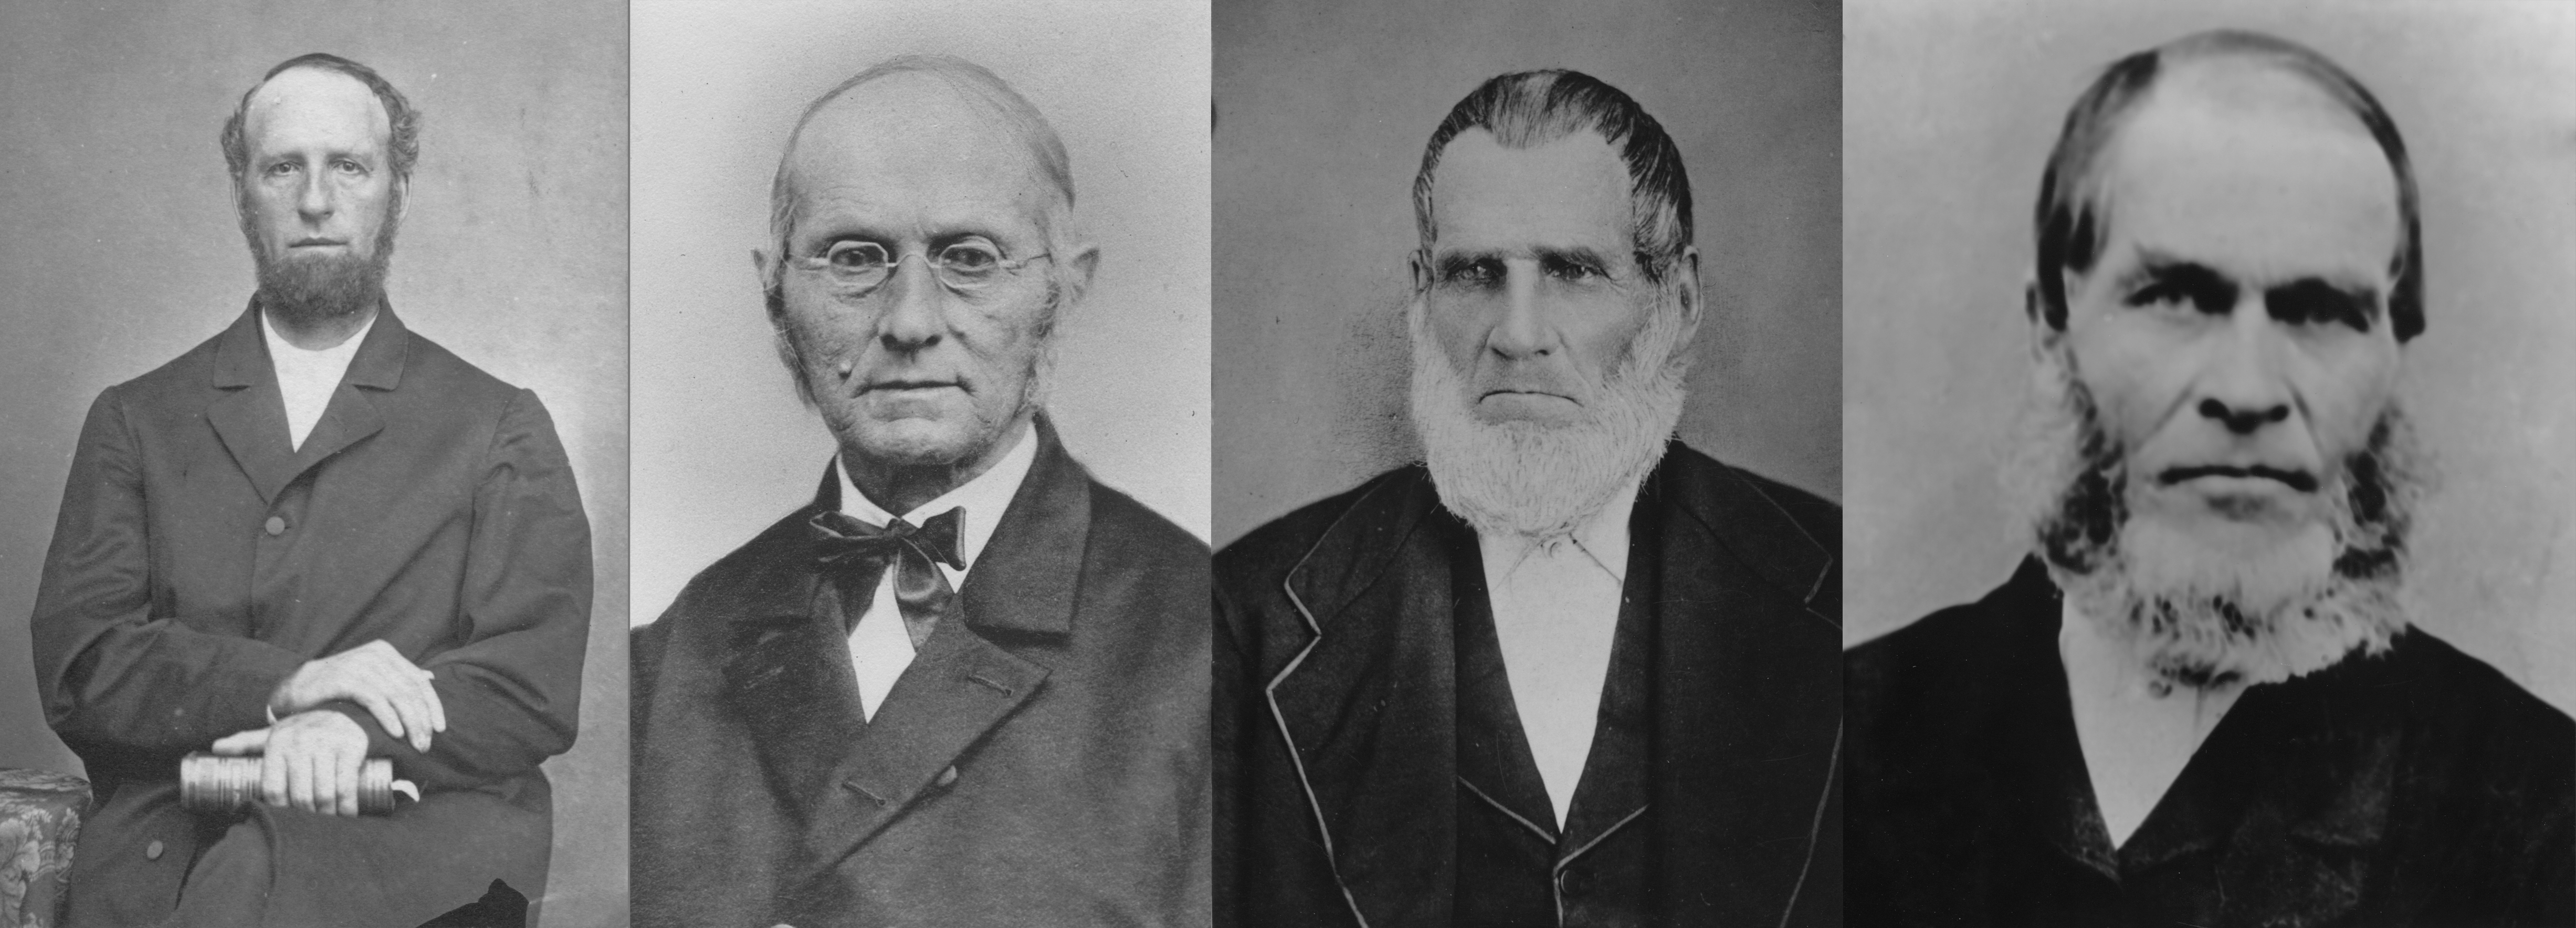
\includegraphics[width=1\linewidth]{images/james-white-joseph-bates-stephen-pierce-hiram-edson.jpg}
    \caption*{James White, Joseph Bates, Stephen Pierce, Hiram Edson}
    \label{fig:pioneers}
\end{figure}


\begin{figure}
    \centering
    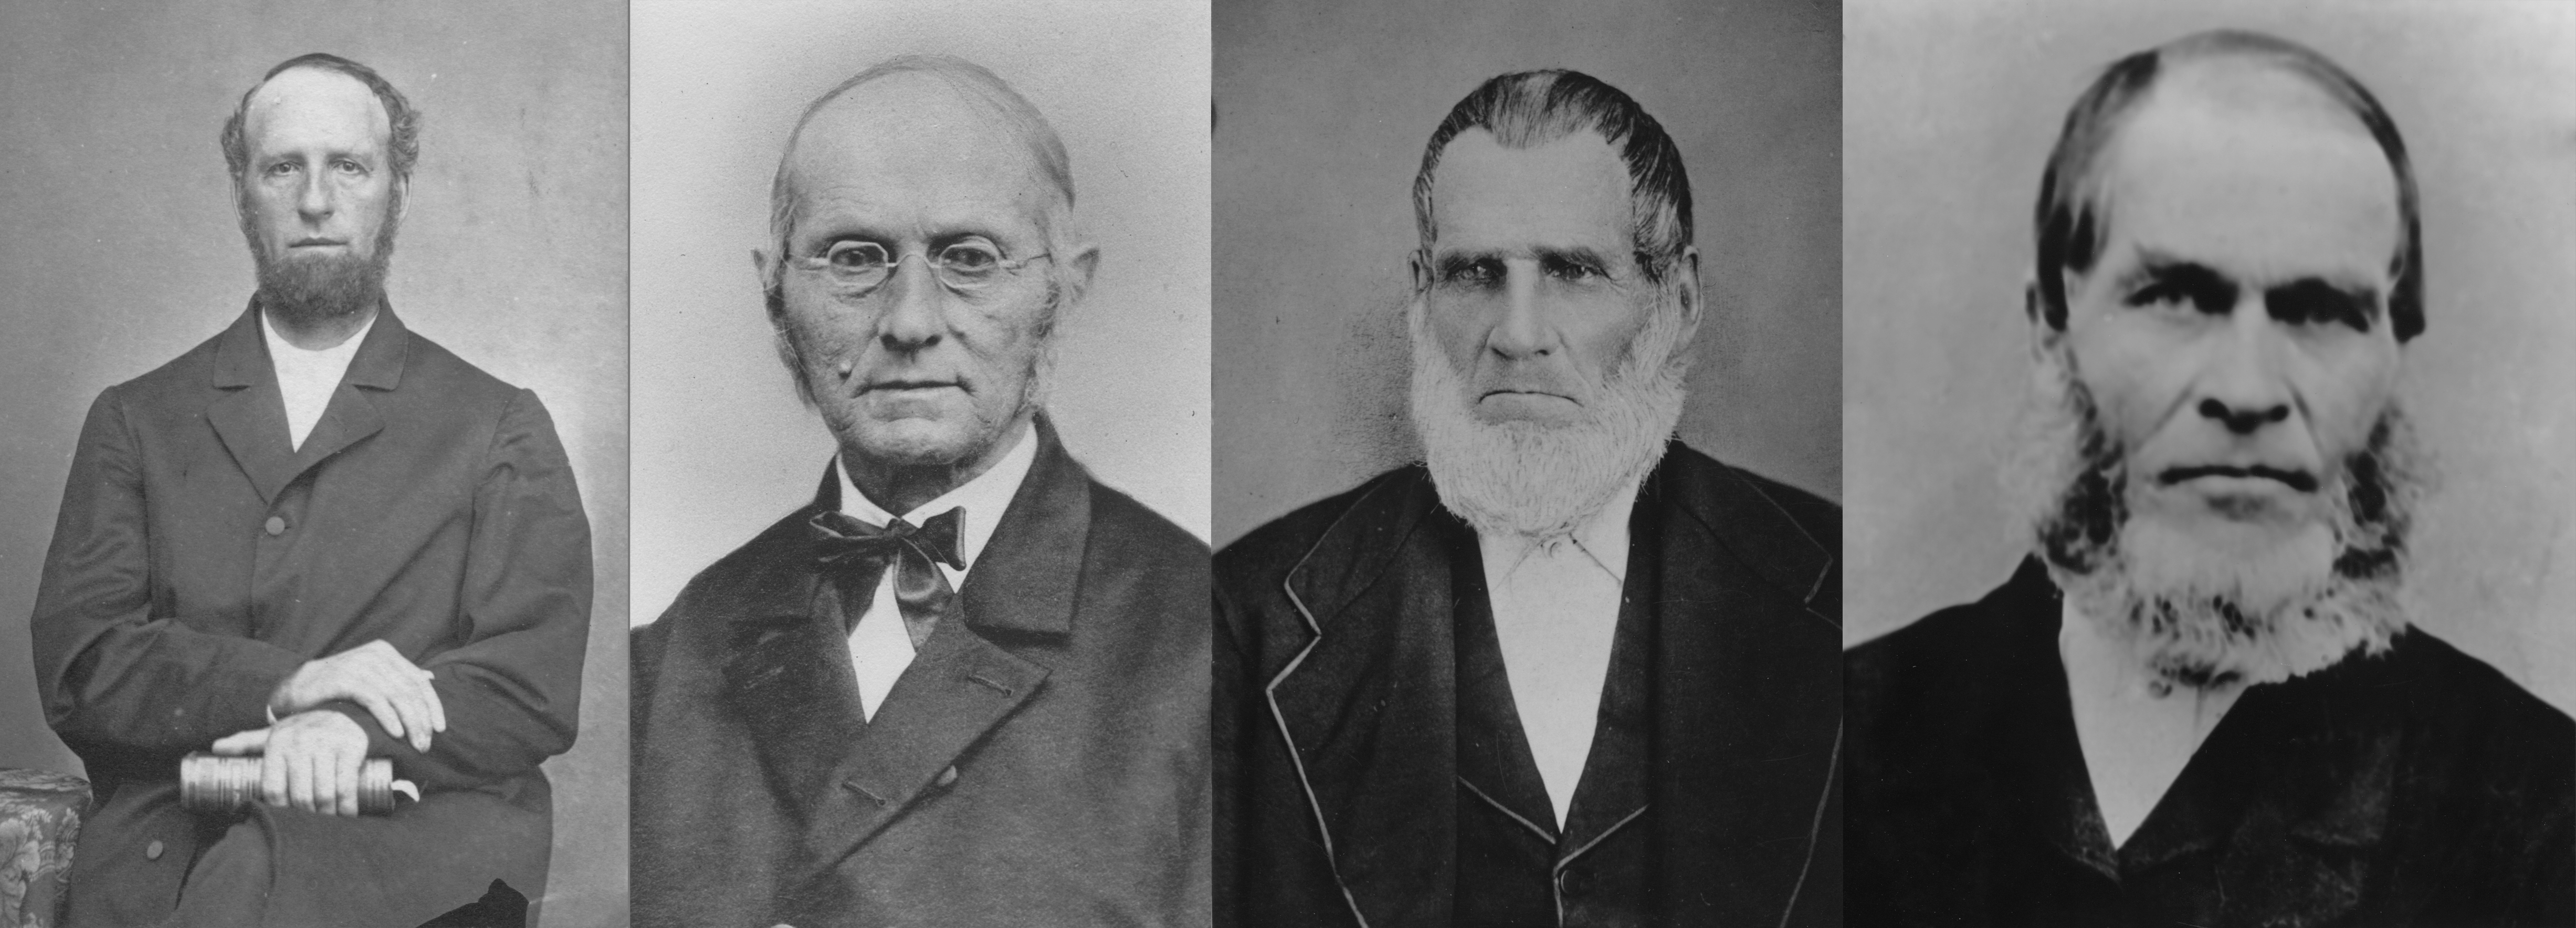
\includegraphics[width=1\linewidth]{images/james-white-joseph-bates-stephen-pierce-hiram-edson.jpg}
    \caption*{جيمس وايت، جوزيف بيتس، ستيفن بيرس، هايرام إدسون}
    \label{fig:pioneers}
\end{figure}


\egwnogap{During this whole time I could not understand the reasoning of the brethren. My mind was locked, as it were, and I could not comprehend the meaning of the scriptures we were studying. This was one of the greatest sorrows of my life. \textbf{I was in this condition of mind until all \underline{the principal points of our faith} were made clear to our minds, in harmony with the word of God}. The brethren knew that when not in vision, I could not understand these matters, and they accepted as light direct from heaven the revelations given.}[SpTB02 57.1; 1904][https://egwwritings.org/read?panels=p417.291]


\egwnogap{خلال هذا الوقت كله لم أستطع فهم تفكير الإخوة. كان عقلي مغلقًا، إن جاز التعبير، ولم أستطع فهم معنى الكتب المقدسة التي كنا ندرسها. كان هذا أحد أعظم أحزان حياتي. \textbf{كنت في هذه الحالة الذهنية حتى تم توضيح جميع \underline{النقاط الرئيسية لإيماننا} لأذهاننا، بما يتوافق مع كلمة الله}. عرف الإخوة أنني عندما لا أكون في رؤيا، لم أستطع فهم هذه الأمور، وقبلوا الإعلانات المعطاة كنور مباشر من السماء.}[SpTB02 57.1; 1904][https://egwwritings.org/read?panels=p417.291]


\egwnogap{For two or three years my mind continued to be locked to an understanding of the Scriptures. In the course of our labors, my husband and I visited Father Andrews, who was suffering intensely with inflammatory rheumatism. We prayed for him. I laid my hands on his head, and said, ‘Father Andrews, the Lord Jesus maketh thee whole.’ He was healed instantly. He got up, and walked about the room, praising God, and saying, ‘I never saw it on this wise before. Angels of God are in this room.’ The glory of the Lord was revealed. Light seemed to shine all through the house, and an angel’s hand was laid upon my head. From that time to this I have been able to understand the word of God.}[SpTB02 57.2; 1904][https://egwwritings.org/read?panels=p417.292]


\egwnogap{لمدة عامين أو ثلاثة أعوام استمر عقلي مغلقًا عن فهم الكتب المقدسة. في سياق أعمالنا، زرت أنا وزوجي الأب أندروز، الذي كان يعاني بشدة من الروماتيزم الالتهابي. صلينا من أجله. وضعت يدي على رأسه، وقلت: “أيها الأب أندروز، الرب يسوع يشفيك”. شُفي على الفور. نهض، ومشى في الغرفة، مسبحًا الله، وقائلاً: “لم أر مثل هذا من قبل. ملائكة الله في هذه الغرفة”. تجلى مجد الرب. بدا النور يشع في جميع أنحاء المنزل، ووُضعت يد ملاك على رأسي. من ذلك الوقت وحتى الآن أصبحت قادرة على فهم كلمة الله.}[SpTB02 57.2; 1904][https://egwwritings.org/read?panels=p417.292]


\egwnogap{\textbf{What influence is it that would lead men at this stage of our history to work in an underhanded, powerful way \underline{to tear down the foundation of our faith},—the foundation that was laid at the beginning of our work by prayerful study of the word and by revelation? Upon \underline{this foundation} we have been building for \underline{the past fifty years}. Do you wonder that when I see the beginning of a work that would \underline{remove some of the pillars of our faith}, I have something to say? I must obey the command, ‘Meet it!’}}[SpTB02 58.1; 1904][https://egwwritings.org/read?panels=p417.295]


\egwnogap{\textbf{ما هو التأثير الذي يدفع الناس في هذه المرحلة من تاريخنا للعمل بطريقة خفية وقوية \underline{لهدم أساس إيماننا}،- الأساس الذي وُضع في بداية عملنا من خلال الدراسة المصلية للكلمة وبالإعلان؟ على \underline{هذا الأساس} كنا نبني \underline{خلال الخمسين سنة الماضية}. هل تتعجبون أنني عندما أرى بداية عمل من شأنه \underline{إزالة بعض أعمدة إيماننا}، يكون لدي ما أقوله؟ يجب أن أطيع الأمر، ‘واجهه!’}}[SpTB02 58.1; 1904][https://egwwritings.org/read?panels=p417.295]


\egwnogap{I have the tenderest feelings toward Dr. Kellogg. For many years I have tried to hold fast to him. God’s word to me has always been, ‘You can help him.’ Sometimes I am awakened in the night, and, rising, I walk the room, praying: ‘O Lord, hold Dr. Kellogg fast. Do not let him go. Keep him steadfast. Anoint his eyes with the heavenly eyesalve, that he may see all things clearly.’ Night after night I have lain awake, studying how I could help him. Earnestly and often I have prayed that the Lord may not permit him to turn away from sanctifying truth. This is the burden that weighs me down,—the desire that he shall be kept from making mistakes that would hurt his soul and \textbf{injure the cause of present truth}. But for some time his actions have revealed that a strange spirit is controlling him. The Lord will take this matter in His own hands. I must bear the messages of warning that God gives me to bear, and then leave with the Lord the results. \textbf{I must now present the matter in all its bearings; for the people of God must not be despoiled}.}[SpTB02 58.2; 1904][https://egwwritings.org/read?panels=p417.296]


\egwnogap{لدي أرق المشاعر تجاه الدكتور كيلوغ. لسنوات عديدة حاولت التمسك به. كلمة الله لي دائمًا كانت: “يمكنك مساعدته”. أحيانًا أستيقظ في الليل، وأنهض، وأمشي في الغرفة، وأصلي: “يا رب، امسك الدكتور كيلوغ بثبات. لا تدعه يذهب. احفظه ثابتًا. امسح عينيه بمرهم العين السماوي، حتى يرى كل الأشياء بوضوح”. ليلة بعد ليلة استلقيت مستيقظة، أدرس كيف يمكنني مساعدته. بجدية وكثيرًا صليت أن الرب لا يسمح له بالابتعاد عن الحق المقدس. هذا هو العبء الذي يثقلني - الرغبة في أن يُحفظ من ارتكاب أخطاء قد تؤذي روحه و\textbf{تضر بقضية الحق الحاضر}. لكن منذ فترة كشفت أفعاله أن روحًا غريبة تسيطر عليه. الرب سيأخذ هذا الأمر في يديه. يجب أن أحمل رسائل التحذير التي يعطيني الله لأحملها، ثم أترك النتائج للرب. \textbf{يجب أن أقدم الآن المسألة بكل جوانبها؛ لأن شعب الله يجب ألا يُسلب}.}[SpTB02 58.2; 1904][https://egwwritings.org/read?panels=p417.296]


\egwnogap{\textbf{We are God’s commandment-keeping people. For the past fifty years every phase of heresy has been brought to bear upon us, to becloud our minds regarding the teaching of the word},\textbf{—especially concerning the ministration of Christ in the heavenly sanctuary, and the message of heaven for these last days, as given by the angels of the fourteenth chapter of Revelation}. \textbf{Messages of every order and kind have been urged upon Seventh-day Adventists, to take the place of the truth which, \underline{point by point}, has been sought out by prayerful study, and testified to by the miracle-working power of the Lord}. \textbf{But \underline{the way-marks} \underline{which have made us what we are}, \underline{are to be preserved}, and they \underline{will be preserved}, as God has signified through His word and the testimony of His Spirit}. \textbf{He calls upon us to \underline{hold firmly}, with the grip of faith, to \underline{the fundamental principles} that are \underline{based upon unquestionable authority}}.}[SpTB02 59.1; 1904][https://egwwritings.org/read?panels=p417.299]


\egwnogap{\textbf{نحن شعب الله حافظو الوصايا. خلال الخمسين سنة الماضية، تم توجيه كل نوع من الهرطقات إلينا، لتشويش أذهاننا بخصوص تعليم الكلمة}،\textbf{—خاصة فيما يتعلق بخدمة المسيح في المقدس السماوي، ورسالة السماء لهذه الأيام الأخيرة، كما أعطاها ملائكة الفصل الرابع عشر من سفر الرؤيا}. \textbf{لقد تم حث رسائل من كل نوع وصنف على الأدفنتست السبتيين، لتحل محل الحق الذي، \underline{نقطة بنقطة}، تم البحث عنه بالدراسة المصلية، وشُهد له بقوة الله العاملة بالمعجزات}. \textbf{لكن \underline{المعالم} \underline{التي جعلتنا ما نحن عليه}، \underline{يجب أن تُحفظ}، وسوف \underline{تُحفظ}، كما أشار الله من خلال كلمته وشهادة روحه}. \textbf{إنه يدعونا إلى \underline{التمسك بقوة}، بقبضة الإيمان، \underline{بالمبادئ الجوهرية} التي \underline{تستند إلى سلطة لا تقبل الشك}}.}[SpTB02 59.1; 1904][https://egwwritings.org/read?panels=p417.299]


There was a necessity to warn the church of the development of the enemy to uproot the foundation of our faith. There was a necessity to remind the church of what constitutes the true foundation of Seventh-day Adventist faith. It seems that Seventh-day Adventists, at that time, were forgetting \egwinline{the way the Lord has led us, and His teaching in our past history.}[LS 196.2; 1915][https://egwwritings.org/read?panels=p41.1083]


كانت هناك ضرورة لتحذير الكنيسة من تطور العدو لاقتلاع أساس إيماننا. كانت هناك ضرورة لتذكير الكنيسة بما يشكل الأساس الحقيقي لإيمان الأدفنتست السبتيين. يبدو أن الأدفنتست السبتيين، في ذلك الوقت، كانوا ينسون \egwinline{الطريقة التي قادنا بها الرب، وتعليمه في تاريخنا الماضي.}[LS 196.2; 1915][https://egwwritings.org/read?panels=p41.1083]


\egw{What influence is it that would lead men at this stage of our history to work in an underhanded, powerful way \textbf{to tear down the foundation of our faith},—the foundation that was laid \textbf{at the beginning of our work} by prayerful study of the word and by revelation? Upon \textbf{this foundation} we have been building for \textbf{the past fifty years}. Do you wonder that when I see the beginning of a work that would \textbf{remove some of the pillars of our faith}, I have something to say? I must obey the command, ‘\textbf{Meet it}!’}[SpTB02 58.1; 1904][https://egwwritings.org/read?panels=p417.295]


\egw{ما هو التأثير الذي يدفع الناس في هذه المرحلة من تاريخنا للعمل بطريقة خفية وقوية \textbf{لهدم أساس إيماننا}،- الأساس الذي وُضع \textbf{في بداية عملنا} من خلال الدراسة المصلية للكلمة وبالإعلان؟ على \textbf{هذا الأساس} كنا نبني \textbf{خلال الخمسين سنة الماضية}. هل تتعجبون أنني عندما أرى بداية عمل من شأنه \textbf{إزالة بعض أعمدة إيماننا}، يكون لدي ما أقوله؟ يجب أن أطيع الأمر، ‘\textbf{واجهه}!’}[SpTB02 58.1; 1904][https://egwwritings.org/read?panels=p417.295]


What was it that Sister White was commanded to meet?


ما الذي أُمرت الأخت وايت بمواجهته؟


\egwinline{About the time that ‘Living Temple’ was published} in the night season she received \egwinline{representations indicating that some danger was approaching,} and that she must \egwinline{prepare for it by writing out the things God has revealed} to her \egwinline{\textbf{regarding the foundation principles of our faith}.}


\egwinline{في الوقت الذي نُشر فيه كتاب ‘ليفينغ تمبل’} في رؤيا ليلية تلقت \egwinline{تمثيلات تشير إلى أن بعض الخطر كان يقترب،} وأنه يجب عليها \egwinline{الاستعداد له من خلال كتابة الأشياء التي كشفها الله} لها \egwinline{\textbf{بخصوص المبادئ الأساسية لإيماننا}.}


She was \egwinline{instructed by the heavenly messenger that some of the reasoning in the book, ‘Living Temple’, is unsound and that \textbf{this reasoning would lead astray} the minds of those who are not thoroughly established on \textbf{the foundation principles} of present truth.}


لقد \egwinline{تلقت تعليمات من الرسول السماوي بأن بعض المنطق في كتاب ‘ليفينغ تمبل’ غير سليم وأن \textbf{هذا المنطق سيضلل} عقول أولئك الذين ليسوا راسخين تمامًا على \textbf{المبادئ الأساسية} للحق الحاضر.}


So, what was the actual problem with the book, “Living Temple”?


إذًا، ما هي المشكلة الفعلية مع كتاب “ذا ليفينغ تمبل”؟


If you are a scholar, or an Adventist historian, or a theologian, or just a student of theology, before you give a straight answer and say that the problem was pantheism, we would like to point you back to the text. Sister White clearly addressed the core issue of the problem stating that the “Living Temple,” \egwinline{introduces that which is naught but speculation in \textbf{regard to the personality of God and where His presence is}.}


إذا كنت عالمًا، أو مؤرخًا أدفنتستيًا، أو لاهوتيًا، أو مجرد طالب لاهوت، قبل أن تعطي إجابة مباشرة وتقول إن المشكلة كانت وحدة الوجود، نود أن نوجهك مرة أخرى إلى النص. لقد تناولت الأخت وايت بوضوح جوهر المشكلة مصرحة أن كتاب “ذا ليفينغ تمبل” \egwinline{يقدم ما هو إلا تخمين فيما \textbf{يتعلق بشخصانية الله وأين وجوده}.}


We do not deny the pantheistic problem of the book, but we want to divert attention from Kellogg’s error to the light God has given. There are two ways to approach Kellogg’s crisis. One is by addressing the pantheism, and another is to address \egwinline{\textbf{the personality of God} and \textbf{where His presence is}}. One way is to study the error, and the other way is to study the Truth. One way is to dissect the darkness and the other way is to drink from the fountain of the Truth. We choose the latter, and for this reason this book is set apart from hundreds of other books written on Kellogg’s crisis. The subject of this book is not pantheism, or any other error, but the truth and what God has revealed about His personality and where His presence is. This was the real issue of Kellogg’s publication.


نحن لا ننكر مشكلة وحدة الوجود في الكتاب، لكننا نريد تحويل الانتباه من خطأ كيلوغ إلى النور الذي أعطاه الله. هناك طريقتان للتعامل مع أزمة كيلوغ. إحداهما من خلال معالجة وحدة الوجود، والأخرى من خلال معالجة \egwinline{\textbf{شخصانية الله} و\textbf{أين وجوده}}. طريقة واحدة هي دراسة الخطأ، والطريقة الأخرى هي دراسة الحق. طريقة واحدة هي تشريح الظلام والطريقة الأخرى هي الشرب من نبع الحق. نحن نختار الأخيرة، ولهذا السبب يتميز هذا الكتاب عن مئات الكتب الأخرى المكتوبة عن أزمة كيلوغ. موضوع هذا الكتاب ليس وحدة الوجود، أو أي خطأ آخر، بل الحق وما كشفه الله عن شخصانيته وأين وجوده. كانت هذه هي القضية الحقيقية لمنشور كيلوغ.


We believe it is a great danger to study and dissect the error because error leads to deception. The problem with deception is that we could be deceived obviously not knowing we are deceived! We firmly believe that Ellen White was the prophet of God and that she was receiving the Light from God \bible{who is light and in Him is no darkness at all}[1 John 1:5]. Therefore, we do not expect Sister White to explain the error in the book, “Living Temple”. Many were coming to her, asking her \egwinline{to explain the positions taken in ‘Living Temple.’} She replied, \egwinline{They are unexplainable}. Her objective was not to dissect the error but to shine the Truth on the \emcap{personality of God} and where His presence is. Thus, she was pointing back to the truths God founded the Seventh-day Adventist Church on. These truths have been constituting the foundation of our faith. These truths have been given to us in our early days. By diverting our attention from the personality of God to pantheism, we are losing an opportunity to remember \egwinline{\textbf{the way the Lord has led us}, and \textbf{His teaching} in our \textbf{past history}}. In this light, we express our concern over the Kellogg crisis and its pantheistic approach, because \egwinline{the track of truth lies close beside the track of error, and both tracks may seem to be one}; the solution to that is to be \egwinline{thoroughly established on \textbf{the foundation principles} of present truth}. Elsewhere, Sister White strongly established this principle.


نعتقد أنه من الخطر الكبير دراسة وتشريح الخطأ لأن الخطأ يؤدي إلى الخداع. المشكلة في الخداع هي أننا قد نُخدع بوضوح دون أن نعرف أننا مخدوعون! نحن نؤمن بقوة أن إلين وايت كانت نبية الله وأنها كانت تتلقى النور من الله \bible{الذي هو نور وليس فيه ظلمة البتة}[1 يوحنا 1:5]. لذلك، لا نتوقع من الأخت وايت أن تشرح الخطأ في كتاب “ذا ليفينغ تمبل”. كان الكثيرون يأتون إليها، ويطلبون منها \egwinline{شرح المواقف المتخذة في ‘ليفينغ تمبل’.} أجابت، \egwinline{إنها غير قابلة للشرح}. لم يكن هدفها تشريح الخطأ بل إلقاء الضوء على \emcap{شخصانية الله} وأين وجوده. وبالتالي، كانت تشير إلى الحقائق التي أسس الله عليها كنيسة الأدفنتست السبتيين. هذه الحقائق كانت تشكل أساس إيماننا. هذه الحقائق أُعطيت لنا في أيامنا الأولى. من خلال تحويل انتباهنا من شخصانية الله إلى وحدة الوجود، نحن نفقد فرصة لتذكر \egwinline{\textbf{الطريقة التي قادنا بها الرب}، و\textbf{تعليمه} في \textbf{تاريخنا الماضي}}. في ضوء ذلك، نعبر عن قلقنا بشأن أزمة كيلوغ ونهجها الوحدوي، لأن \egwinline{مسار الحق يقع بالقرب من مسار الخطأ، وقد يبدو كلا المسارين واحدًا}؛ الحل لذلك هو أن نكون \egwinline{راسخين تمامًا على \textbf{المبادئ الأساسية} للحق الحاضر}. في مكان آخر، أسست الأخت وايت هذا المبدأ بقوة.


\egw{Satan is by no means asleep; he is wide-awake and is playing the game of life for the souls of the people of God. He will come to them with flattery of all kinds, in the hope of leading them to swerve from their allegiance. \textbf{He desires to call their attention from the real issues to false theories}.}[Ms132-1903.42; 1904][https://egwwritings.org/read?panels=p9056.56]


\egw{الشيطان ليس نائمًا بأي حال من الأحوال؛ إنه مستيقظ تمامًا ويلعب لعبة الحياة من أجل نفوس شعب الله. سيأتي إليهم بإطراء من كل الأنواع، على أمل قيادتهم للانحراف عن ولائهم. \textbf{إنه يرغب في لفت انتباههم من القضايا الحقيقية إلى النظريات الكاذبة}.}[Ms132-1903.42; 1904][https://egwwritings.org/read?panels=p9056.56]


So, let us focus our attention on the real issue instead of the false theories.


لذلك، دعونا نركز انتباهنا على القضية الحقيقية بدلاً من النظريات الكاذبة.


% The Foundation of our Faith

\begin{titledpoem}
    \stanza{
        Pillars of truth, laid with care, \\
        By pioneers who sought in prayer. \\
        Principles firm, the Lord's design, \\
        A platform strong, for all time.
    }

    \stanza{
        Beware the subtle shifts that call, \\
        To change what should not change at all. \\
        Our identity, in these we find, \\
        God's revelations to mankind.
    }

    \stanza{
        Stand fast upon this solid ground, \\
        Where wisdom and God's light abound. \\
        Defend these truths with all your might, \\
        For in them shines eternal light.
    }
\end{titledpoem}